%%% LaTeX Template
%%% This template can be used for both articles and reports.
%%%
%%% Copyright: http://www.howtotex.com/
%%% Date: February 2011

%%% Preamble
\documentclass[paper=a4, fontsize=11pt]{scrartcl}	% Article class of KOMA-script with 11pt font and a4 format


\usepackage[italian]{babel}															% English language/hyphenation
\usepackage[protrusion=true,expansion=true]{microtype}				% Better typography
\usepackage{amsmath,amsfonts,amsthm}										% Math packages
\usepackage[pdftex]{graphicx}														% Enable pdflatex
%\usepackage{color,transparent}													% If you use color and/or transparency
\usepackage[hang, small,labelfont=bf,up,textfont=it,up]{caption}	% Custom captions under/above floats
\usepackage{epstopdf}																	% Converts .eps to .pdf
\usepackage{subfig}																		% Subfigures
\usepackage{booktabs}																	% Nicer tables
\usepackage[latin1]{inputenc}
\usepackage{listings}
\usepackage{xcolor}
\lstdefinestyle{sharpc}{language=[Sharp]C, frame=lr, rulecolor=\color{blue!80!black}}

  \usepackage{courier}

%%% Advanced verbatim environment
\usepackage{verbatim}
\usepackage{fancyvrb}
\DefineShortVerb{\|}								% delimiter to display inline verbatim text


%%% Custom sectioning (sectsty package)
\usepackage{sectsty}								% Custom sectioning (see below)
\allsectionsfont{%									% Change font of al section commands
	\usefont{OT1}{bch}{b}{n}%					% bch-b-n: CharterBT-Bold font
%	\hspace{15pt}%									% Uncomment for indentation
	}

\sectionfont{%										% Change font of \section command
	\usefont{OT1}{bch}{b}{n}%					% bch-b-n: CharterBT-Bold font
	\sectionrule{0pt}{0pt}{-5pt}{0.8pt}%	% Horizontal rule below section
	}


%%% Custom headers/footers (fancyhdr package)
\usepackage{fancyhdr}
\pagestyle{fancyplain}
\fancyhead{}														% No page header
\fancyfoot[C]{\thepage}										% Pagenumbering at center of footer
\renewcommand{\headrulewidth}{0pt}				% Remove header underlines
\renewcommand{\footrulewidth}{0pt}				% Remove footer underlines
\setlength{\headheight}{13.6pt}

%%% Equation and float numbering
\numberwithin{equation}{section}															% Equationnumbering: section.eq#
\numberwithin{figure}{section}																% Figurenumbering: section.fig#
\numberwithin{table}{section}																% Tablenumbering: section.tab#


\definecolor{pblue}{rgb}{0.13,0.13,1}
\definecolor{pgreen}{rgb}{0,0.5,0}
\definecolor{pred}{rgb}{0.9,0,0}
\definecolor{pgrey}{rgb}{0.46,0.45,0.48}


\usepackage{color}
\usepackage{xcolor}
\usepackage{listings}

 \lstset{
         basicstyle=\footnotesize\ttfamily, % Standardschrift
         %numbers=left,               % Ort der Zeilennummern
         numberstyle=\tiny,          % Stil der Zeilennummern
         %stepnumber=2,               % Abstand zwischen den Zeilennummern
         numbersep=5pt,              % Abstand der Nummern zum Text
         tabsize=2,                  % Groesse von Tabs
         extendedchars=true,         %
         breaklines=true,            % Zeilen werden Umgebrochen
         keywordstyle=\color{red},
    		frame=b,         
 %        keywordstyle=[1]\textbf,    % Stil der Keywords
 %        keywordstyle=[2]\textbf,    %
 %        keywordstyle=[3]\textbf,    %
 %        keywordstyle=[4]\textbf,   \sqrt{\sqrt{}} %
         stringstyle=\color{white}\ttfamily, % Farbe der String
         showspaces=false,           % Leerzeichen anzeigen ?
         showtabs=false,             % Tabs anzeigen ?
         xleftmargin=17pt,
         framexleftmargin=17pt,
         framexrightmargin=5pt,
         framexbottommargin=4pt,
         %backgroundcolor=\color{lightgray},
         showstringspaces=false      % Leerzeichen in Strings anzeigen ?        
 }
\lstloadlanguages{% Check Dokumentation for further languages ...
         %[Visual]Basic
         %Pascal
         %C
         %C++
         %XML
         %HTML
         %Java
{[Sharp]C}
 }
\usepackage{caption}
\DeclareCaptionFont{white}{\color{white}}
\DeclareCaptionFormat{listing}{\colorbox{gray}{\parbox{\textwidth}{#1#2#3}}}
\captionsetup[lstlisting]{format=listing,labelfont=white,textfont=white}

%%% Title	
\title{ \vspace{-1in} 	\usefont{OT1}{bch}{b}{n}
		\huge \strut Implementazione di Finding Triangles con Hadoop MapReduce\strut \\
		\Large \bfseries \strut Sistemi di elaborazione di grandi quantit\`a di dati 20013 \strut
}
\author{ 									\usefont{OT1}{bch}{m}{n}
        Nicola Febbrari\\		\usefont{OT1}{bch}{m}{n}
        Universit\`a degli Studi di Verona\\	\usefont{OT1}{bch}{m}{n}
        Facolt\`a MM.FF.NN.\\
        \texttt{nicola.febbrari@studenti.univr.it}
}
\date{13 gennaio 2014}

%%% Begin document
\begin{document}
\maketitle
\section{Introduzione}
Lo scopo del progetto \`e quello di implementare un algoritmo per calcolare il numero di triangoli presenti in un grafo, utilizzando le tecniche di MapReduce e il Framework Haddop.


\section{Il problema}
L'analisi dei dati e da sempre uno dei provessi aziendali chiave per la vita

I social network negli ultimi anni hanno avuto una notevole diffusione, l'aumento esponenziale del numero di utenti che interagistcono con questi sistemi 
ha avuto come diretta conseguenza un  incremento della quantit\`a di dati che devono essere registrati, gestiti ed ovviamente elaborati.
Il businnes ha subito capito quanto fossero imprtanti tutte queste informazioni e per questo motivo negli ultimi c'\'e stato un grosso hype su come sia 
possibile recuperare, elaborare e dedurre nuove informazioni a partire da una base di informazioni enorme.

Una caratteristica molto interessante di un grafo che rappresenta un soocial network e' il numero di triangoli contenuti in sesso. 
Il numero di questi triangoli rapportato al totale dei nodi che costituiscono il grafo \'e un indice di quanto sia SOCIAL il grafo che rappresenta il social network. (anzianit\'a della comunity)
Tipicamente dati 3 nodi (A,B,C) in un grafo, dato un nodo  A che si relaziona sia con B che con C, nel grafo viene a formarsi un triangolo se esiste anche la relazione che lega B-C.

\section{Strumenti e Framework}
\paragraph{Sistema}
Apache Hadoop \`e un framework opensource utilizzato per l' elaborazione di grandi quantit\`a di dati. 
Si basa su MapReduce, un paradigma di programmazione parallela con il quale \'e possibile realizzare algoritmi applicabili a sitemi distributi e con alto grado di scalabilit\`a.

\paragraph{Sviluppo}
L'implementazione dell 'algoritmo di Finding Triangles  \'e stata realizzata scrivedo un programma Java che utilizza ed estende le Hadoop API di Base.
\paragraph{Testing}
Come suite di testing \`e stato utilizzato MRUnit una libreria Java che consente di fare Unit test sui jobs di MapReduce.
\paragraph{UI}
Come tool di supporto \`e stato utilizzato Hue, un' inerfaccia web-based per la gestione ed il monitoraggio del file sistem di Hadoop (HDFS) e dei jobs MapReduce.
\paragraph{Versioning}
Come sistema di versioning \`e stato utilizzato GitHub, un servizio web che utilizza la piattaforma GIT.
\paragraph{Sorgente dati}
Come sistema di versioning \`e stato utilizzato GitHub, un servizio web che utilizza la piattaforma GIT.


\section{Implementazioni}
\subsection{Algoritmo 2 Jobs}
L'algoritmo a 2 Jobs prevede un prima fase in cui vengono elaborate tutte le relazioni e viene creata in output la combinazione di tutti i possibili triangoli a meno dell'ultimo arco necessario per chiudere il triangolo.\\
Esempio date le relazioni A - K, K - B e A - B  (in cui A<K<B ) il Job 1 elabora le relazioni in cui K \'e nodo in un caso maggiore o minore unendo queste relazioni trova al coppia A - B che verr\'a cercate nel Job2. Se questa relazione \'e presente allora esiste sicuramente il atriangolo A K B


\begin{figure}[h]
\centering
        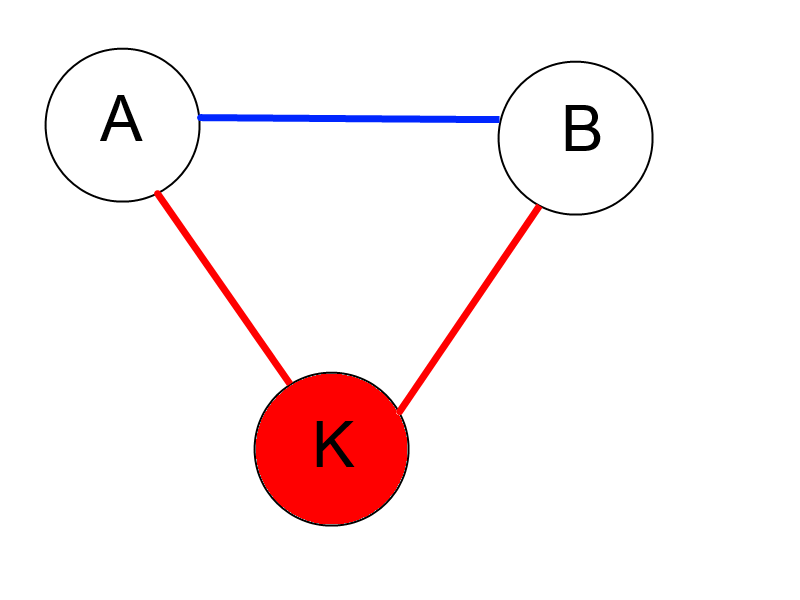
\includegraphics[totalheight=6cm]{Graph1.png}
    \caption{Il Job 1 elabora le relazioni rosse in cui K  in un caso \`e nodo  maggiore e nell altro caso minore. Il Job2 cerca la relazione blu A B.}
    \label{fig:verticalcell} 
\end{figure}
\paragraph{Job1 Mapper}
Nella parte di mapper del primo Job come prima cosa escludo tutti gli archi che portano nello stesso nodo e poi definisco le relazioni solamente come da nodo minore a nodo maggiore in modo da evitare duplicazioni. La definizione di triangolo in un grafo non prende in considerazione la direzione delle relazioni fra i nodi e nel mio caso i nodi sono rappresentati da dei valori Long, quindi la relazione di ordinamento \`e immediata.\\ 
In questa fase per ogni relazione mando in output 2 oggetti <<VALUE1,BOOL>,VALUE2>. Come KEY (<VALUE1,BOOL>) del VALUE (VALUE2) che passo al reducer uso un dato strutturato contenente il nodo e un valore booleano che identifica se il nodo VALUE \`e un nodo minore o maggiore di quello della KEY secondo la relazione di ordinamento definita. 

\lstset{
language=Java,
  showspaces=false,
  showtabs=false,
  breaklines=true,
  showstringspaces=false,
  breakatwhitespace=true,
  commentstyle=\color{pgreen},
  keywordstyle=\color{pblue},
  stringstyle=\color{pred},
  basicstyle=\ttfamily,
  moredelim=[il][\textcolor{pgrey}]{$$},
  moredelim=[is][\textcolor{pgrey}]{\%\%}{\%\%}
}
\begin{lstlisting}[label=Mapper1,caption=Implementazione del Mapper1]
@Override
	public void map(LongWritable key, Text value, Context context)
			throws IOException, InterruptedException {
		String line = value.toString();
		String[] sp = line.split("\s+");// splits on TAB
		Long lp0=Long.parseLong(sp[0]);
		Long lp1=Long.parseLong(sp[1]);
		if (lp0!= lp1) { 	//exclude self relation
			if (lp0 < lp1) {
				textP.set(lp1, false);
				text.set(lp0);
				context.write(textP, text);// "0" link_from
				textP.set(lp0, true);
				text.set(lp1);
				context.write(textP, text);// "1" link_to
			} else {
				textP.set(lp0, false);
				text.set(lp1);
				context.write(textP, text);// "0" link_from

				textP.set(lp1, true);
				text.set(lp0);
				context.write(textP, text);// "1" link_to
			}
		}
}\end{lstlisting}
\paragraph{Job1 Reducer}

Per suddividere correttamente tutti gli elementi prodotti dal Mapper sono stati ridefiniti il SortComparator e il GroupingComparator.
Il nuovo GroupingComparator ragruppa le chiavi valutando solamente il valore del nodo chiave K e garantendo che tutte le relazioni che contengono K come nodo maggiore o come nodo minore vengano elaborate dallo stesso reducer. Il SortComparator ridefinito invece ordina gli elementi in base al valore del nodo chiave K e in caso di uguale nodo chiave mette prima gli elementi con valore booleano false nella chiave.\\ Il reducer  garzie all'ordinamento esamina prima tutte le relazioni in cui il nodo chiave \'e nodo maggiore, queste coppie (nodo valore - nodo chiave) salvati in una lista L. Una volta che tutte le relazioni in cui il nodo chiave \'e nodo maggiore sono finite inizieranno le relazioni in cui il nodo chiave \'e nodo minore. Per ognuna di queste nuove relazioni (es. K-B) il reducer cicla la lista L mandando in output per ogni elemento (A-K) in L una relazione (A-B, K). Infatti la presenza della relazione A-B nel grafo chiuderebbe il triangolo A-K-B 

Il redoucer, grazie alla redifinizione del GroupinComparator1 (ragruppa le chiavi valutando solamente il valore del nodo della chiave) e  del Comparator1 (ordina le chiavi mettendo prima quelle con valore false ) tutti gli output del task di Map. Prima salva in una lista l'elenco dei nodi padre del nodo chiave, una volta che tutti i nodi sono stati ciclati, per ogni nodo figlio, scrive in output la terna di valori con la coppia nodo padre - nodo figlio che completerebbe il triangolo.
\begin{lstlisting}[label=Reducer1,caption=Implementazione del Reducer1]	
	@Override
	protected void reduce(LongBit key, Iterable<LongWritable> values, Context context)
			throws IOException, InterruptedException {
		partialJoin.clear();
		LongWritable k = key.getFirst();

		for (LongWritable valText : values) {
			Long val = valText.get();
			if (!key.getSecond().get())// link from
			{
				if (!partialJoin.contains(val))
					partialJoin.add(val);
			} else // link to
			{
				WriteContext(k, context, val);
			}
		}
	}
\end{lstlisting}
\paragraph{Job2 Mapper}
Nella secondo Job l'output del primo Job viene unito nuovamente alla sorgente dati iniziale. Il secondo mapper in questo scorre l'unione dei 2 input, nel caso la relazione \'e una relazione presente nel grafo iniziale scrive in output un elemento ((A,B,false),0) se invece \'e generata dal Job 1 scrive in output  ((A,B,true),K) dove A,B sono nodi della relazione e K \'e nodo intermedio fra A e B calcolato da Job1.
\paragraph{Job2 Reducer}
Il secondo reducer ridefinendo in modo analogo al Reducer1 sia il SortComparator che il GroupingComparator scorre l'input prima cerca le relazioni AB che chiuderebbero un triangolo e poi per ogni relazione generata dal Job1 con output AB manda in output AKB.

\subsection{Algoritmo single Job}
L'algoritmo a Job singolo \'e molto pi\'u complesso del precedente.
L'idea \'e quella di costruire una suddivisione delle relazioni in input nei vari reducer definendo delle chiavi strutturate e abbinate ai vari task di Reduce. Questa suddivisione viene realizzata con una Hash sul valore del nodo stesso.
Ogni trinagolo \'e formato da  3 nodi (x,y,z) i quali sono legati dalle relazioni A=(x,y), B=(x,z) e C=(y,z). In base a questo una relazione pu\'o essre una delle 3 relazioni che compongono il triangolo, quindi dato R=(u,v), R pu\'o essere una relazione di tipo A e quindi  il triangolo sarebbe (u,v,?) oppure di tipo B con (u,?,v) o C con (?,u,v).

Il task di Map divide le relazioni in input in tante parti quante le possibili casistiche in cui la relazione pu\'o essere utilizzata per completare un triangolo. 
La suddivisione viene fatta grazie ad una funzione di hash che

compiti. Supponiamo che un compito Map \'e dato tupla E (u, v) per inviare ad alcuni
Ridurre i compiti. In primo luogo, pensare a (u, v) come una tupla del join termine E (X, Y). noi
pu\'o hash u e v per ottenere i numeri della benna per X e Y, ma noi non so
il secchio per cui Z hash. Quindi, dobbiamo mandare E (u, v) per tutte le attivit\'a riduttore
che corrisponde ad una sequenza di tre numeri benna .. h (u), h (v), z per qualsiasi
della b possibili secchi z.


To begin, assume that the nodes of a graph are numbered 1, 2, . . . , n. We
use a relation E to represent edges. To avoid representing each edge twice,
we assume that if E(A,B) is a tuple of this relation, then not only is there
an edge between nodes A and B, but also, as integers, we have A < B.3
This requirement also eliminates loops (edges from a node to itself), which we
generally assume do not exist in social-network graphs anyway, but which could
lead to triangles that really do not involve three different nodes.
Using this relation, we can express the set of triangles of the graph whose
edges are E by the natural join
To understand this join, we have to recognize that the attributes of the relation
E are given different names in each of the three uses of E. That is, we imagine
there are three copies of E, each with the same tuples, but with a different
schemas. In SQL, this join would be written using a single relation E(A,B) as
follows:
SELECT e1.A, e1.B, e2.B
FROM E e1, E e2, E e3
WHERE e1.A = e2.A AND e1.B = e3.A AND e2.B = e3.B
In this query, the equated attributes e1.A and e2.A are represented in our join
by the attribute X. Also, e1.B and e3.A are each represented by Y ; e2.B and
e3.B are represented by Z.
Notice that each triangle appears once in this join. The triangle consisting
of nodes v1, v2, and v3 is generated when X, Y , and Z are these three nodes in
numerical order, i.e., X < Y < Z. For instance, if the numerical order of the
nodes is v1 < v2 < v3, then X can only be v1, Y is v2, and Z is v3.
The technique of Section 2.5.3 can be used to optimize the join of Equation
10.1. Recall the ideas in Example 2.9, where we considered the number
of ways in which the values of each attribute should be hashed. In the present
example, the matter is quite simple. The three occurrences of relation E surely
have the same size, so by symmetry, attributes X, Y , and Z will each be hashed
to the same number of buckets. In particular, if we hash nodes to b buckets,
then there will be b3 reducers. Each Reduce task is associated with a sequence
of three bucket numbers (x, y, z), where each of x, y, and z is in the range 1 to
b.
The Map tasks divide the relation E into as many parts as there are Map
tasks. Suppose one Map task is given the tuple E(u, v) to send to certain
Reduce tasks. First, think of (u, v) as a tuple of the join term E(X, Y ). We
can hash u and v to get the bucket numbers for X and Y , but we don t know
the bucket to which Z hashes. Thus, we must send E(u, v) to all Reducer tasks
that correspond to a sequence of three bucket numbers ..h(u), h(v), z for any
of the b possible buckets z.
But the same tuple E(u, v) must also be treated as a tuple for the term
E(X,Z). We therefore also send the tuple E(u, v) to all Reduce tasks that
correspond to a triple ..h(u), y, h(v) for any y. Finally, we treat E(u, v) as a
tuple of the term E(Y,Z) and send that tuple to all Reduce tasks corresponding
to a triple ..x, h(u), h(v) for any x. The total communication required is thus
3b key-value pairs for each of the m tuples of the edge relation E. That is, the
minimum communication cost is O(mb) if we use b3 Reduce tasks.
Next, let us compute the total execution cost at all the Reduce tasks. Assume
that the hash function distributes edges sufficiently randomly that the
Reduce tasks each get approximately the same number of edges. Since the total
number of edges distributed to the b3 Reduce tasks is O(mb), it follows that each
task receives O(m/b2) edges. If we use the algorithm of Section 10.6.2 at each
Reduce task, the total computation at a task is O..(m/b2)3/2, or O(m3/2/b3).
Since there are b3 Reduce tasks, the total computation cost is O(m3/2), exactly
as for the one-processor algorithm of Section 10.6.2.\\
\begin{lstlisting}[label=Mapper,caption=Implementazione del Mapper single Job]
	@Override
	public void map(LongWritable key, Text value, Context context)
			throws IOException, InterruptedException {

		Configuration conf = context.getConfiguration();
		this.buckets = conf.getInt("b",3);
		
		String line = value.toString();
		line = line.replaceAll("^\\s+", "");
		String[] sp = line.split("\\s+");// splits on TAB
		Long lp0 = Long.parseLong(sp[0]);
		Long lp1 = Long.parseLong(sp[1]);
		if (lp0 != lp1) {
			if (lp0 < lp1) {
				SetContext(context, lp0, lp1);
			} else {
				SetContext(context, lp1, lp0);
			}
		}
	}

	private void SetContext(Context context, Long lp0, Long lp1)
			throws IOException, InterruptedException {
		to.set(lp1);
		for (long j = 0; j < buckets; j++) {
			context.write(new LongLongLongLong("A",lp0 % buckets, lp1 % buckets, j, lp0), to);// "1"
			context.write(new LongLongLongLong("B",lp0 % buckets, j, lp1 % buckets, lp0), to);// "1"
			context.write(new LongLongLongLong("C",j, lp0 % buckets, lp1 % buckets, lp0), to);// "1"
		}
	}
\end{lstlisting}


\begin{lstlisting}[label=Reducer,caption=Implementazione del Reducer single Job]
	@Override
	protected void reduce(LongLongLongLong key, Iterable<LongWritable> values,
			Context context) throws IOException, InterruptedException {
		//partialJoin.clear();
		List<Long> tmpList = new LinkedList<Long>();

		for (LongWritable valText : values) {
			Long from = key.getfourth().get();
			Long to = valText.get();
			Pair<Long, Long> p = CreatePair(to, from);
			if (partialJoin.containsKey(p)	&& key.getRel().toString().equals("C")) {
				WriteContext(partialJoin.get(p), context);
				partialJoin.remove(p);
			}
			for (Long tmpTo : tmpList) {
				Pair<Long, Long> l = CreatePair(to, tmpTo);
				if (!to.equals(tmpTo) && key.getRel().toString().equals("B")) {
					Triplet<Long, Long, Long> t  = new Triplet<Long, Long, Long>(from, l.getValue0(),l.getValue1());
					if(partialJoin.containsKey(l)){
						if(!partialJoin.get(l).contains(t))
							partialJoin.get(l).add(t);
					}
					else{
						List<Triplet<Long, Long, Long>> lt= new LinkedList<Triplet<Long, Long, Long>>();
						lt.add(new Triplet<Long, Long, Long>(from, l.getValue0(),l.getValue1()));						
						partialJoin.put(l,lt);						
					}
						
				}
			}
			if (!tmpList.contains(to)&& key.getRel().toString().equals("A")) {
				tmpList.add(to);
			}
		}
	}
\end{lstlisting}

\paragraph{Ottimizzazioni}


\section{Complessit\`a}
\paragraph{Algoritmo 2 Jobs}
\paragraph{Algoritmo Single Jobs}


\section{Osservazioni}

\end{document}